% !TEX root = SystemTemplate.tex

\chapter{System  and Unit Testing}

This section describes the approach taken with regard to system and unit testing. 

\section{Overview}
The testing approach for this project was a bit different from traditional software testing. We did not have an automated testing framework to run unit tests or regression tests, instead we verified visually when a piece of the project was behaving as expected. This project used many off the shelf hardware and software products where testing the functionality of these pieces has already been done by the manufacturer of that technology. The tests described below allowed us to evaluate whether or not the different subsystems of the UAV were functioning correctly.

\section{Dependencies}
There were no testing frameworks used for this project. All testing was verified manually.

\newpage
\section{Test Setup and Execution}
\subsection{Testing: U-1}
\textbf{As a user, I want to communicate the waypoints to the UAV.}\\
\begin{tabular}{| c | >{\raggedright}m{4cm} | m{4cm} | c |}\hline
	Task No. & Task & Test & Completed\\\hline
	3 & Modify mission communication implementation as necessary & User is able to create mission file with ground control station. & Yes\\\hline
	3 & Modify mission communication implementation as necessary & User is able to load mission file on offboard(ODroid). & Yes\\\hline
	3 & Modify mission communication implementation as necessary & Landing Algorithm on offboard starts after completing last mission. & Yes\\\hline
\end{tabular}
\vfill
Creating mission files from the ground control station was completed using the QGroundControl software. Once GPS way-points were set up a mission file could be generated. A figure showing the use of QGroundControl is below.
\begin{figure}[H]
	\centering
	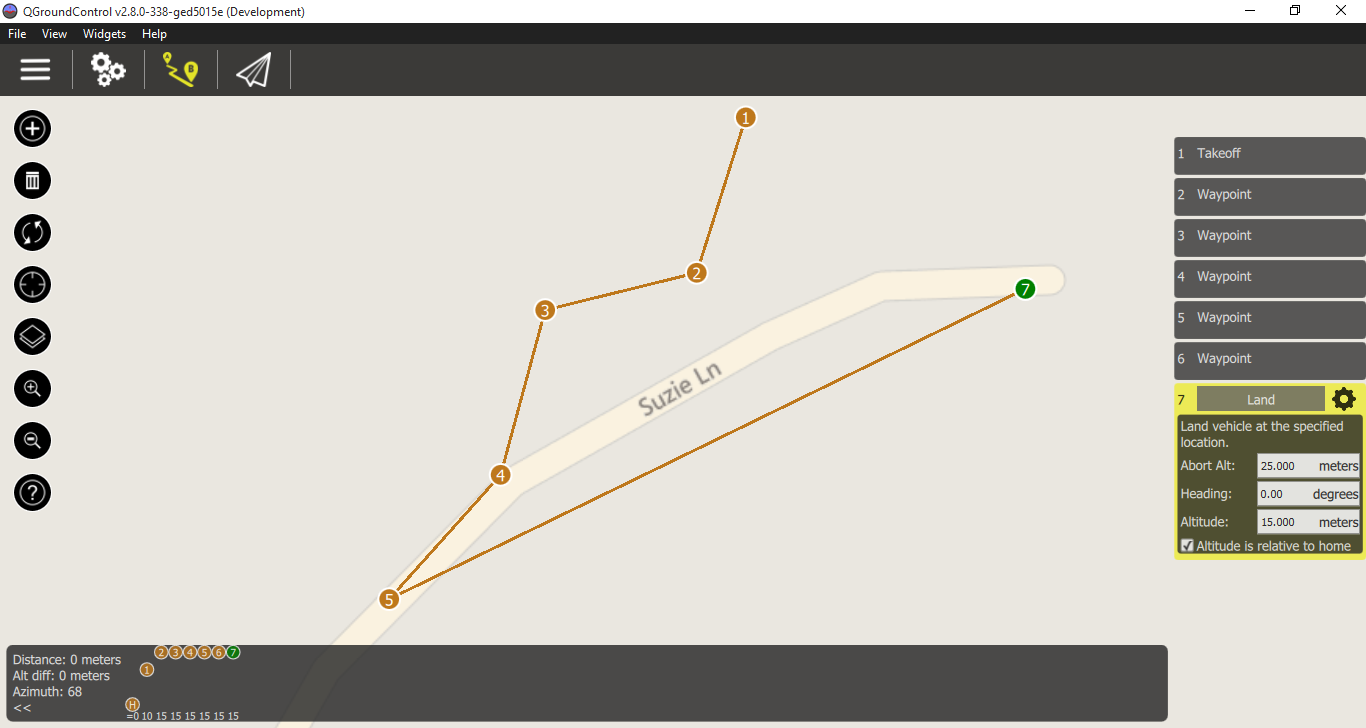
\includegraphics[width=\textwidth]{images/route1.PNG}
	\caption{QGroundControl mission creation.}
\end{figure}

\newpage
\subsection{Testing: O-1}
\textbf{As an owner, I want the UAV to autonomously take-off from the landing pad.}\\
\begin{tabular}{| c | >{\raggedright}m{4cm} | m{4cm} | c |}\hline
	Task No. & Task & Testing & Completed\\\hline
	3 & Modify/Rewrite take-off implementation as necessary
 & FCU recieves take-off mission from mission from offboard control. & Yes\\\hline	
	3 & Modify/Rewrite take-off implementation as necessary
 & FCU executes take-off mission. & Yes\\\hline	
\end{tabular}
\vfill
Similar to the previous user story, autonomous takeoff was handled by the flight controller in conjunction with the mission planner. In the previous figure you can see a mission in the QGroundControl software. What is not as obvious as the way-points on the map is the list of events to be executed on the right side of the screen. As you can see in the figure below, autonomous take-off is part of the mission file generated and uploaded to the ODroid.

\begin{figure}[H]
\centering
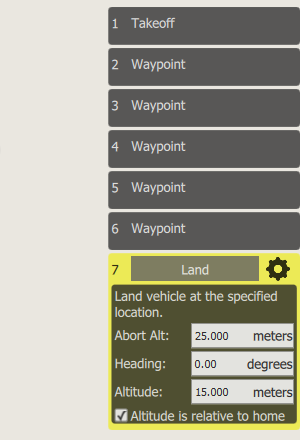
\includegraphics[height=0.8\textwidth]{images/events.PNG}
\caption{QGroundControl showing autonomous takeoff event.}
\end{figure}

\newpage
\subsection{Testing: O-2}
\textbf{As an owner, I want the UAV to autonomously navigate through a set of waypoints.}\\
\begin{tabular}{| c | >{\raggedright}m{4cm} | m{4cm} | c |}\hline
	Task No. & Task & Test & Completed\\\hline
	3 & Modify/Rewrite waypoint navigation implementation as necessary & FCU receives navigation missions from offboard control. & Yes\\\hline
	3 & Modify/Rewrite waypoint navigation implementation as necessary & FCU executes navigation in sequence. & Yes\\\hline
	3 & Modify/Rewrite waypoint navigation implementation as necessary & FCU follows, reasonably, the planned navigation. & Yes\\\hline
\end{tabular}
\vfill
As can been seen in the previous two figures QGroundControl was able to handle the autonomous takeoff and way-point navigation of the UAV. What remained to be tested was our UAV's ability to execute these missions. This was tested by uploading missions to off-board control (ODROID) and letting them be run. There are videos showing the UAV perform the autonomous takeoff and way-point navigation which verify that the UAV was able to perform those operations. Finally we needed to ensure the UAV followed the GPS way-points 'reasonably' well so we measured the error in the UAV's target landing location. As you can see from the picture below the UAV was able to land within 18 inches of its target using only GPS.

\begin{figure}[H]
\centering
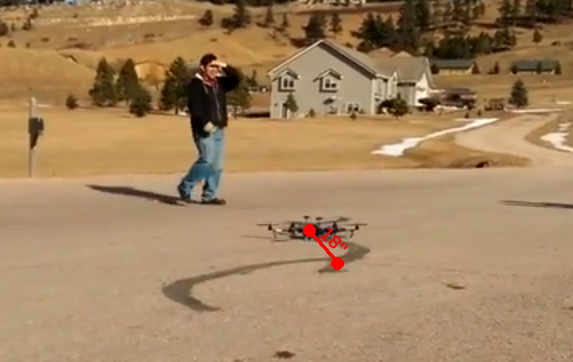
\includegraphics{images/UAVLanding}
\caption{UAV landing error.}
\end{figure}

\newpage
\subsection{Testing: O-3}
\textbf{As an owner, I want the UAV to autonomously return to the location of the landing pad.}\\
\begin{tabular}{| c | >{\raggedright}m{4cm} | m{4cm} | c |}\hline
	Task No. & Task & Test & Completed\\\hline
	3 & Modify navigate to landing waypoint implementation as necessary & FCU receives last navigation mission from offboard control. & Yes\\\hline
	3 & Modify navigate to landing waypoint implementation as necessary & FCU executes navigation mission. & Yes\\\hline
	3 & Modify navigate to landing waypoint implementation as necessary & FCU navigates within a reasonable distance(\textless 10m) to waypoint. & Yes\\\hline
\end{tabular}

In order to return to the location of the landing pad, the mission must specify the final GPS way-point as the starting way-point. This was done and verified by actual flight that can be seen in this \href{https://www.youtube.com/watch?v=wye3LynE1CM}{YouTube video.}

\newpage
\subsection{Testing: O-4}
\textbf{As an owner, I want the UAV to autonomously land on the landing pad without damaging the craft}\\
\begin{tabular}{| c | >{\raggedright}m{4cm} | m{4cm} | m{4cm} | m{4cm} |}\hline
	Task No. & Task & Test & Completed\\\hline
	4 & Modify landing pose implementation as necessary & UAV accurately estimates pose of AR tag & Yes\\\hline
	4 & Modify landing pose implementation as necessary & UAV centers over AR tag within (\textless 0.1m). & No\\\hline
	4 & Modify landing pose implementation as necessary & The UAV remains centered during descent within (\textless 0.1m). & No\\\hline
	4 & Modify landing pose implementation as necessary & The UAV lands without damaging craft or legs. & No\\\hline
\end{tabular}

\vfill
Although we were not able to test the physical UAVs ability to react to the AR Tag we were able to get AR Tag tracking up and running. The AR Tag tracking was able to accurately estimate the pose of an AR Tag within 15 ft. A demonstration of this tracking is shown below.
\begin{figure}[H]
\centering
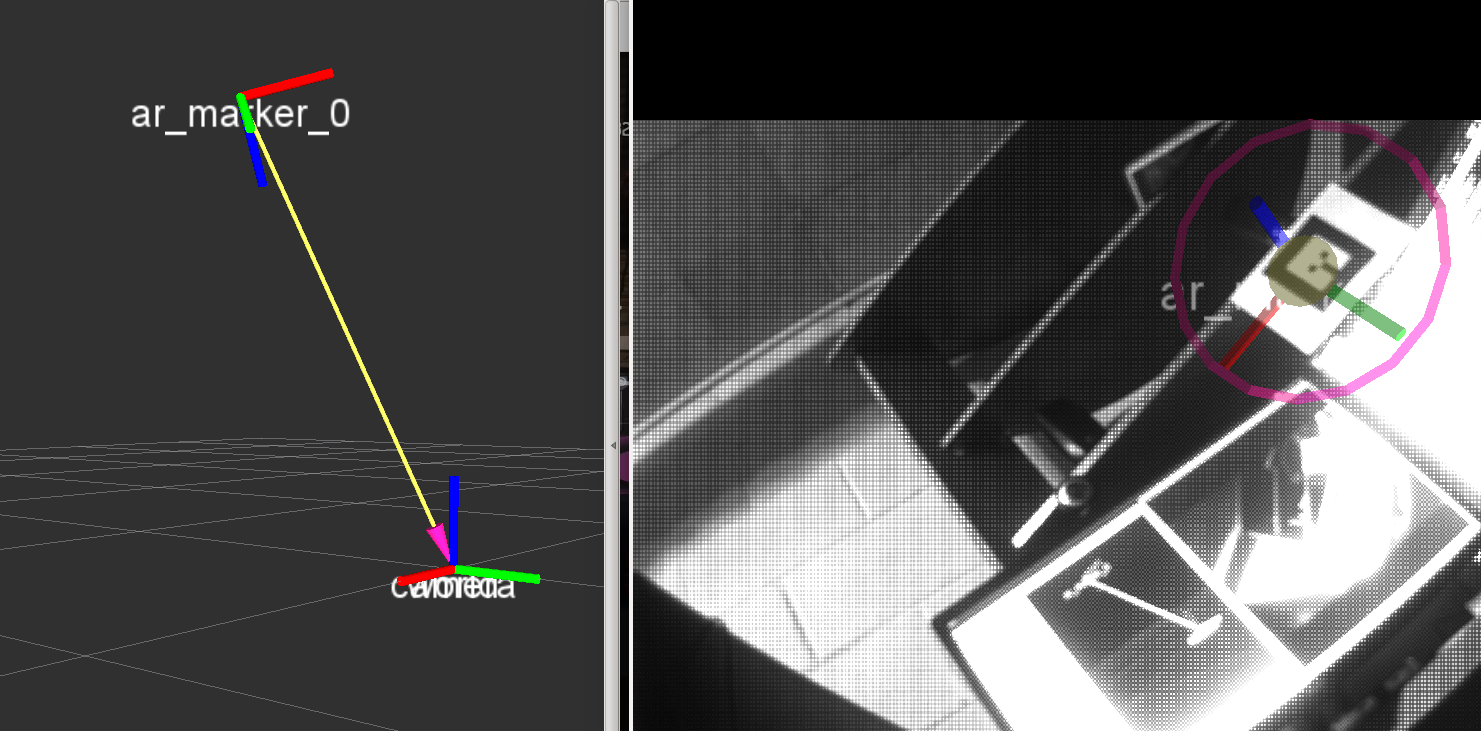
\includegraphics[width=\textwidth]{images/poseEstimation.png}
\caption{AR Tag tracking with AR Track ALVAR}
\end{figure}

\newpage
\subsection{Testing: O-5}
\textbf{As an owner, I want the UAV to autonomously land on the landing pad with the correct orientation.}\\
\begin{tabular}{| c | >{\raggedright}m{4cm} | m{4cm} | m{4cm} |}\hline
	Task No. & Task & Test & Completed\\\hline
		4 & Modify landing orientation implementation as necessary & UAV accurately estimates the orientation of AR tag & Yes\\ \hline
		4 & Modify landing orientation implementation as necessary & UAV changes orientation to align with AR tag, within 15$\deg$ & No\\ \hline
		4 & Modify landing orientation implementation as necessary & UAV maintains correct orientation during descent within 15$\deg$ & No\\ \hline
\end{tabular}

\vspace{4cm}
On this final user story we were only able to complete the first task which is a common task between this user story and the previous one (O-4). Which to reiterate is the correct pose estimation of an AR Tag. If you would like to see the results of the AR Tracking look at the previous page.

